\section{Reinforcement Learning}
Mainly from OpenAIs \textit{Introduction to RL} \cite{rl-openai}.
\subsection{Key Concepts and Terminology}
\begin{figure}
\centering
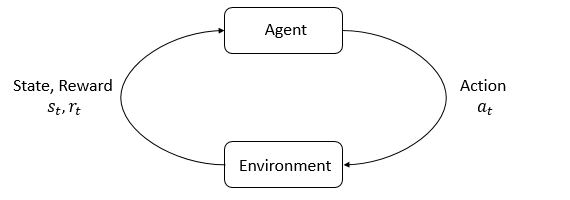
\includegraphics[scale=0.8]{rl/agent-environment}
\caption{Agent-environment interaction loop.}\label{fig:agent-env}
\end{figure}

\paragraph{State $s$} Complete description of world state.

\paragraph{Observation $o$} (partial) description of the world state (depends if environment is \textit{fully} or \textit{partially} observed.

\paragraph{Action space} Set of valid actions in a given environment. Can be either \textit{discrete} or \textit{continuous}.

\paragraph{Policy $a_t$} Rule used by an agent to decide what actions to take. Can be eiter deterministic ($a_t = \mu_{\theta}(s_t)$) or stochastic ($a_t \sim \pi_{\theta}(\cdot|s_t)$), where $\theta$ indicates used function parameters. Most common kinds of stochastic policies:
\begin{enumerate}
    \item
        \textbf{Categorial} (for discrete AS): like a classifier over discrete actions.
        \begin{itemize} 
            \item
                Sampling: Straight forward
            \item
                Log-Likelihood: $log_{\pi_{\theta}}(a|s) = log[P_{\theta}(s)]_a$, where $P_{\theta}(s)$ is the last layer of probabilities.
        \end{itemize}
    \item
        \textbf{Diagonal Gaussian} (for continuous AS): has a neural network that maps from observations to mean actions, $\mu_{\theta}(s)$, describing a multivariate normal distribution with mean vector $\mu_{\theta}(s)$ and diagonal covariance matrix $\Sigma$ (log-vector of standard deviations, either hyperparameter or also computed by neural network).
        \begin{itemize}
            \item
                Sampling: With $z \sim \mathcal{N}(0, I)$, $a = \mu_{\theta}(s) + \sigma_{\theta}(x) \odot z$
            \item
                Log-Likelihood: See \cite{rl-openai}
        \end{itemize}
\end{enumerate}
\paragraph{Trajectories (episodes, rollouts)} Sequence of states and actions in the world, $\tau = (s_0, a_0, s_1, a_1, \dots)$. $s_0$ is randomly sampled from \textbf{start-state-distribution} $\rho_0(\cdot)$. State transitions follow the natural laws of the environment (can also be either deterministic or stochastic) and depend only on the most recent $a_t$ and the last state $s_t$.

\paragraph{Reward and Return} $r_t$ is either $R(s_t, a_t, s{t+1})$, $R(s_t)$ or $R(s_t, a_t)$ (different dependencies). The goal of the agent is to maximize some notion of cumulative reward over a trajectory.
\begin{enumerate}
    \item
        Finite-horizon undiscounted return: $R(\tau) = \sum_{t=0}^T r_t$
    \item
        Infinite-horizon discounted return: $R(\tau) = \sum_{t=0}^{\infty} \gamma^t r_t$. 'Cash now is better than cash later', with discount factor and under reasonable conditions the infinite sum converges.
\end{enumerate}

\paragraph{The RL Problem} The goal in RL is to select a policy which maximizes \textbf{expected return} when the agent acts according to it. Suppose both environment transitions and policy are stochastic, probability of a $T$-step trajectory is: 
$$P(\tau | \pi) = \rho_0(s_0) \prod_{t=0}^{T-1} P(s_{t+1} | s_t, a_t) \pi(a_t | s_t).$$
The exted return $J(\pi)$ (for whichever measure) is then: 
$$J(\pi) = \int_{\tau} P(\tau | \pi) R(\tau) = E_{\tau \sim \pi}[R(\tau)].$$
The central optimization problem in RL can be expressed by:
$$\pi^* = \argmax_{\pi} J(\pi).$$

\paragraph{Value functions} It is often useful to know the value (expected return, infinite discounted horizon) of a state, or state-action pair, after which acted according to a particular policy. 
\begin{enumerate}
    \item
        \textbf{On-Policy Value Function} $V^{\pi}(s)$ 
    \item
        \textbf{On-Policy Action-Value Function} $Q^{\pi}(s,a)$ 
    \item
        \textbf{Optimal Value Function} $V^{*}(s)$ 
    \item
        \textbf{Optimal Action-Value Function} $Q^*(s,a)$ (optimal because acting according to optimal policy)
\end{enumerate}
Important key connections between value and action-value function:
\begin{enumerate}
    \item
        $V^{\pi}(s) = E_{a \sim \pi} [Q^{\pi}(s,a)]$
    \item
        $V^*(s) = \max_{a} Q^*(s,a)$
\end{enumerate}

\paragraph{Optimal Q-Function and Optimal Action}
